\documentclass[twoside]{article}
\usepackage{preamble_style}
\usepackage{preamble}
\usepackage{bibliography}


\title{Numerical study of the\\2D Kuramoto-Sivashinsky equation}
\author{Víctor Ballester Ribó}
\date{\parbox{\linewidth}{\centering
Instabilities and Nonlinear Phenomena\endgraf
M2 - Applied and Theoretical Mathematics\endgraf
Université Paris-Dauphine, PSL\endgraf
\today}}


\begin{document}
\maketitle
\begin{abstract}
  The aim of this report is to give both qualitative and quantitative insight into the chaotic behaviour of the 2D Kuramoto-Sivashinsky equation. This equation is more commonly known in its 1D version and this report wants to complement the numerical study carried out in \cite{Kalogirou2015} in order to extend the bibliography on the 2D version of the equation. Kuramoto-Sivashinsky types of equations are seen in various physical phenomena such as flame propagation or reaction-diffusion systems \cite{Kuramoto,Sivashinsky1977}. We will see that the 2D KS equation exhibits chaotic behaviour as we increase the spatial domain size.
\end{abstract}
% {
% \hypersetup{linkcolor=black}
% \tableofcontents
% }

\section{Introduction}\label{sec:intro}
The well-known 1D Kuramoto-Sivashinsky (KS) equation can be written as
\begin{equation}
  u_t + \frac{1}{2} {u_x}^2 + u_{xx} + u_{xxxx} = 0
\end{equation}
It is usually equipped with periodic boundary conditions $u(t, x + L) = u(t, x)$ for some $L > 0$, which defines the domain of definition of the PDE, and an initial condition $u(0, x) = u_0(x)$ \cite{1d-ks}. The natural extension in the 2D case is the following Dirichlet problem with periodic boundary conditions:
\begin{equation}
  \begin{cases}
    u_t + \frac{1}{2} \abs{\grad u}^2 + \laplacian u + \laplacian^2 u = 0 & \text{in } (0, \infty) \times [0, L_x) \times [0, L_y) \\
    u(t, x, y) = u(t, x + L_x, y)                                         & \text{in } [0, \infty) \times \RR \times [0, L_y)      \\
    u(t, x, y) = u(t, x, y + L_y)                                         & \text{in } [0, \infty) \times [0, L_x) \times \RR      \\
    u(0, x, y) = u_0(x, y)                                                & \text{for all } x \in [0, L_x), y \in [0, L_y)
  \end{cases}
\end{equation}
with $L_x, L_y > 0$. For the sake of simplicity, we will rescale the variables in order to obtain a fixed square domain of definition, namely:
\begin{equation}
  x_\mathrm{new} = \frac{2\pi}{L_x} x \qquad y_\mathrm{new} = \frac{2\pi}{L_y} y \qquad t_\mathrm{new} = {\left(\frac{L_x}{2 \pi}\right)}^2 t
\end{equation}
Using this new variables (and dropping the subscript \emph{new} for simplicity), the equation becomes:
\begin{equation}\label{eq:2d_ks}
  \begin{cases}
    u_t + \frac{1}{2} \abs{\grad_\nu u}^2 + \laplacian_\nu u + {\laplacian_\nu}^2 u = 0 & \text{in } (0, \infty) \times [0, 2\pi) \times [0, 2\pi) \\
    u(t, x, y) = u(t, x + 2\pi, y)                                                      & \text{in } [0, \infty) \times \RR \times [0, 2\pi)       \\
    u(t, x, y) = u(t, x, y + 2\pi)                                                      & \text{in } [0, \infty) \times [0, 2\pi) \times \RR       \\
    u(0, x, y) = u_0(x, y)                                                              & \text{for all } x \in [0, 2\pi), y \in [0, 2\pi)
  \end{cases}
\end{equation}
where we used the notation from \cite{Kalogirou2015}:
\begin{align}
  \grad_\nu & = \left(\partial_x , \sqrt{\frac{\nu_2}{\nu_1}} \partial_y
  \right)   & \div_\nu                                                   & = \partial_x + \sqrt{\frac{\nu_1}{\nu_2}} \partial_y
  \\ \laplacian_\nu &= \div_\nu(\grad_\nu) = \partial_{xx} + \frac{\nu_2}{\nu_1} \partial_{yy} & {\laplacian_\nu}^2 &= \laplacian_\nu(\laplacian_\nu) := {\partial_{x}}^4 + 2 \frac{\nu_2}{\nu_1} {\partial_{x}}^2{\partial_{y}}^2 + \frac{{\nu_2}^2}{{\nu_1}^2} {\partial_{y}}^4
\end{align}
and $\nu_1 :={\left( \frac{L_x}{2\pi} \right)}^2$, $\nu_2 := {\left( \frac{L_y}{2\pi} \right)}^2$. Note that the new equation is invariant under the transformation $(t,x,y, \nu_1, \nu_2) \mapsto \left( \frac{\nu_2}{\nu_1} t, y, x, \nu_2, \nu_1 \right)$ if and only if the initial condition is symmetric in $x$ and $y$. In that case, if $u(t,x,y)$ is a solution of the equation with parameters $(\nu_1, \nu_2)$, then $u\left( \frac{\nu_2}{\nu_1} t, y, x \right)$ is the solution of the equation with parameters $(\nu_2, \nu_1)$.

Let's study now the linear stability of the different modes $(k_x, k_y)$ of the equation for $k_x,k_y\in\NN\cup\{0\}$. Setting $v = \delta(e^{\lambda t+i(k_x x + k_y y)} + \cc)$, with $\delta \ll 1$ and $\cc$ denoting the complex conjugate, as a perturbation of the trivial state $u = 0$, we obtain the following equality once we impose that $v$ is a solution of \cref{eq:2d_ks}:
\begin{equation}\label{eq:linear_stability}
  \lambda = \left({k_x}^2+ \frac{\nu_2}{\nu_1} {k_y}^2\right)\left( 1 - \nu_1{k_x}^2 - \nu_2{k_y}^2\right)
\end{equation}
We see that, for example, if $\nu_1, \nu_2 \geq 1$, then there is no pair $(k_x, k_y)$ that makes $\lambda > 0$ and therefore all the nodes are stable. But as soon as we decrease $\nu_1$ or $\nu_2$ below $1$, unstable nodes start to appear in an \emph{increasing}\footnote{Increasing in the sense the node $(k_x+1,k_y)$ will become unstable once the node $(k_x,k_y)$ had become unstable and not before. The same applies for the $y$-direction.} order. For example, for $\nu_1=\nu_2=1/6$ the nodes $(0,1)$, $(1,0)$, $(1,1)$, $(2,0)$, $(0,2)$, $(2,1)$, $(1,2)$ are unstable and all the others are stable.

In order to contribute to the bibliography on the 2D KS equation, we will study the equation with an initial condition different from the one used in \cite{Kalogirou2015}, which was $u_0(x,y) = \sin(x) + \sin(y) + \sin(x+y)$. Instead, we will use the following initial condition:
\begin{equation}\label{eq:initial_condition}
  u_0(x,y) = \sin(x) + \sin(y) + \cos(x+y) + \sin(4x+4y) + \cos(7x) + \cos(7y)
\end{equation}
which is still symmetric in $x$ and $y$. Note that we are adding the modes $(4,4)$, $(7,0)$ and $(0,7)$ to the initial condition used in \cite{Kalogirou2015} and so a richer behaviour is expected.

In order to distinguish and classify the different kinds of behaviour that the equation exhibits, we will monitor the $L^2$-norm of the solution:
\begin{equation}
  E(t):=\norm{u(t)}_{L^2}^2 = \int_0^{2\pi} \int_0^{2\pi} {u(t,x,y)}^2 \dd{x} \dd{y}
\end{equation}
It will be of interest to study also its time derivative $\dot{E}(t)$ and the phase space $(E(t), \dot{E}(t))$ (see \cref{sec:types_of_solutions} for more details).

Finally, we can easily note that the mean of the solution is decreasing in time. Indeed:
\begin{multline}
  4\pi^2\dv{\overline{u}}{t}= \int_0^{2\pi} \int_0^{2\pi} u_t \dd{x} \dd{y} = -\int_0^{2\pi} \int_0^{2\pi} \left( \frac{1}{2} \abs{\grad_\nu u}^2 + \laplacian_\nu u + {\laplacian_\nu}^2 u \right) \dd{x} \dd{y} =\\= -\frac{1}{2}\int_0^{2\pi} \int_0^{2\pi} \left({u_x}^2 + \frac{\nu_2}{\nu_1} {u_y}^2\right) \dd{x} \dd{y} \leq 0
\end{multline}
where we used the fact that the solution is periodic in $x$ and $y$. If we forget about the trivial state $u=0$ or any other stationary state, this later inequality is strict and so the mean of the solution is strictly decreasing in time. In order to avoid this, we will subtract the mean of the solution at each step of integration, or equivalently, we will solve the equation
\begin{equation}
  u_t + \frac{1}{2} \left[\abs{\grad_\nu u}^2 - \frac{1}{4\pi^2}\int_0^{2\pi} \int_0^{2\pi} \abs{\grad_\nu u}^2 \dd{x} \dd{y} \right] + \laplacian_\nu u + {\laplacian_\nu}^2 u = 0
\end{equation}
with the same initial condition as before, because we have chosen an initial condition with zero mean. The reader may notice that here we have used the same notation to denote the initial solution and $u-\overline{u}$, but it should be clear from the context which one we are referring to.
\section{Numerical methods}

There are several numerical methods to integrate this kind of nonlinear equations. In this report we will use a pseudo-spectral method. The idea is to divide the spatial grid $[0,2\pi]\times [0,2\pi]$ in $N_x \times N_y$ cells and to approximate the solution $u(t,x,y)$ by a truncated Fourier series in each cell:
\begin{equation}\label{eq:idft}
  \tilde{u}(t,x_i,y_j) = \sum_{k_x=-N_x/2}^{N_x/2-1} \sum_{k_y=-N_y/2}^{N_y/2-1} \hat{u}(t,k_x,k_y) e^{i(k_x x_i + k_y y_j)}
\end{equation}
for $i=0,\dots,N_x-1$ and $j=0,\dots,N_y-1$. The coefficients $\hat{u}(t,k_x,k_y)$ are the discrete Fourier coefficients of the solution, and they are given by:
\begin{equation}\label{eq:dft}
  \hat{u}(t,k_x,k_y) = \frac{1}{N_x N_y} \sum_{i=0}^{N_x-1} \sum_{j=0}^{N_y-1} u(t,x_i,y_j) e^{-i(k_x x_i + k_y y_j)}
\end{equation}
To efficiently compute the discrete Fourier transform, we will use the Fast Fourier Transform (FFT) algorithm, which reduces the complexity of the computation from $\mathcal{O}({N_x}^2 {N_y}^2)$ to $\mathcal{O}(N_x N_y \log(N_x N_y))$ and attains its maximum performance when $N_x$ and $N_y$ are powers of $2$.

To integrate the PDE in time, we discretize the time domain $[0,T]$ in $N_t$ points separated by a time step $h$. We will use a family of schemes that treat the linear part implicitly and the nonlinear part explicitly, the so called IMEX schemes \cite{Akrivis_kuramoto}. The general theory of IMEX schemes was introduced in \cite{Akrivis2004}, in which they consider schemes of the form
\begin{equation}\label{eq:nonlinear_pde}
  u_t+\mathcal{L}u=\mathcal{N}(u)
\end{equation}
where $\mathcal{L}$ is a linear operator and $\mathcal{N}$ is a nonlinear operator. In order for the scheme to be stable and convergent, we need to check the conditions given in \cite{Akrivis2004}. These require $\mathcal{L}$ being a self-adjoint and positive definite operator and $\mathcal{N}$ being a locally Lipschitz continuous operator. In our problem, $\mathcal{L}=\laplacian_\nu + {\laplacian_\nu}^2$ but in this case, the operator is not positive definite (see \cite{phdthesis_anna} for explicit details). However, adding a large enough constant $c$ to both sides of the equation solves the problem. We will not reproduce the proof of $\mathcal{N}u=-\frac{1}{2} \abs{\grad_\nu u}^2 + cu$ being locally Lipschitz continuous, as it is not the main interest of this report, and it can be found in \cite{Akrivis_kuramoto}. The constant $c$ that makes the scheme stable and convergent is $c=1+\frac{1}{\nu_1}$ \cite{phdthesis_anna}.

That being set, we will use the 2nd order backward differentiation formula (BDF2) as the scheme to integrate our equation in the Fourier space. We have chosen BDF2 schemes because backward differentiation of order 1 (implicit Euler) produced inconsistencies for small values of $\nu_1$ and $\nu_2$, and higher orders of backward differentiation require much more time to compute. In the Fourier space, \cref{eq:nonlinear_pde} becomes, using matrix notation:
\begin{equation}
  \vf{\tilde{u}}_t+\vf{L}\vf{\tilde{u}}=\vf{N}(\vf{\tilde{u}})
\end{equation}
The IMEX-BDF2 scheme for \cref{eq:nonlinear_pde} is given by:
\begin{equation}
  \frac{3}{2} \vf{\tilde{u}}^{n+2} +h \vf{L} \vf{\tilde{u}}^{n+2} = 2 \vf{\tilde{u}}^{n+1} - \frac{1}{2} \vf{\tilde{u}}^{n} + 2h \vf{N}(\vf{\tilde{u}}^{n+1}) -  h \vf{N}(\vf{\tilde{u}}^{n})
\end{equation}
from which we can iteratively solve using the initial condition as a zero step and a IMEX-BDF1 scheme as a first step:
\begin{equation}
  \vf{\tilde{u}}^{n+1} + h \vf{L} \vf{\tilde{u}}^{n+1} = \vf{\tilde{u}}^{n} + h \vf{N}(\vf{\tilde{u}}^{n})
\end{equation}
Recall that in practice \cref{eq:dft} has to be approximated with $\tilde{u}(t_k,x_i,y_j)$ instead of using the unknown quantity $u(t_k,x_i,y_j)$, where $t_k$ is the $k$-th time step.

For the majority of the simulations, we have used $N_x=N_y=64$, which corresponds to a spatial resolution of $dx=dy=2\pi/64\approx 0.098$. The time step used was $h=0.005$, although for some computations, specially those more chaotic, we have decrease it to $h=0.001$. All the code used in this report has been written in C, using the FFTW library \cite{fftw} to compute the FFT, and it can be found in this \href{https://github.com/victorballester7/2d-kuramoto-sivashinsky}{GitHub} repository. The reader may want to check that link to see some of the animations that we have produced, in order to better understand the different types of behaviour that we will describe in the next section.

\section{Results}
In this section we will present the main results of this report.
\subsection{Types of solutions}\label{sec:types_of_solutions}
We will start by presenting the different types of solutions that we can find for the 2D KS equation and how we can detect them.

The most simple type of solution are the stationary states. These can be characterized by observing a constant energy evolution in time as well as constant point on the discretized grid where the maximum of the solution is attained. This last characterization will be of interest for easily distinguishing between time-periodic waves and travelling waves.

There are few different types of periodic solutions. We start with the travelling waves, which are solutions of the form $u(t,x,y) = f(x-ct,y-dt)$, where $c,d\in\RR$ are the speeds of the wave in the $x$ and $y$ directions respectively. They are characterized by the periodic oscillations of the position of a point on the grid, say for convention $u(t,\pi,\pi)$, and a line pattern in the plot $\argmax_x u(t,x,y)$ vs $\argmax_y u(t,x,y)$, which will give the direction of the front of the wave. A different kind of waves are the time-periodic waves, which also exhibit a periodic variation of $u(t,\pi,\pi)$ but the plot $\argmax_x u(t,x,y)$ vs $\argmax_y u(t,x,y)$ does not show any line pattern. In this case the energy of the solution exhibits a periodic behaviour which can be confirmed with a periodic orbit in the phase space $(E(t), \dot{E}(t))$. Finally, we have periodic bursts. These are characterized by an almost constant behaviour of the energy between one or more states together with periodic abrupt and rapid changes in the energy that make the energy jump from one state to another. We want to make clear that when we find only one state in the energy, which may correspond to several physical states, we will call it a periodic homoclinic burst. Whereas if we find more than one state in the energy, and therefore more than one physical state, we will call it a periodic heteroclinic burst. In both cases, the energy will be almost constant between bursts (see \cref{sec:periodic_bursts} for visual examples).

Finally, we have the chaotic or almost chaotic solutions. The one closest to the group above are the quasi-periodic solutions, which can be easily recognized by observing at the return maps $(E_n,E_{n+1})$ where $E_n$ is the energy at time $t_n$ which is the $n$-th intersection of the orbit in the phase space $(E(t), \dot{E}(t))$ with the transversal section $\dot{E}(t)=0$. In these plots we observe a dense set of points that form a continuous curve, differently from the periodic solutions where we observe only a few isolated points. We should make a note on how did we manage to find the zeros of $\dot{E}$. As suggested in \cite{Kalogirou2015}, we used a 2nd order linear interpolation polynomial using 3 consecutive points of $\dot{E}$ and then approximating the zero of $\dot{E}$ by the zero of the interpolation polynomial. Two other kinds of chaotic solutions are the chaotic homoclinic and heteroclinic burst, which resemble their analogous periodic solutions but with a disrupted anomaly periodicity just before each burst (see \cref{sec:chaotic} for examples).

\subsection{General results}\label{sec:general_results}
As done in \cite{Kalogirou2015} we will also perform a general computation to understand the behaviours for all the values of $\nu_1$ and $\nu_2$ in the interval $[0,1]$ with a discretization of $0.05$. The results are shown in \cref{fig:classification_nu1_nu2}.

\begin{figure}[ht]
  \centering
  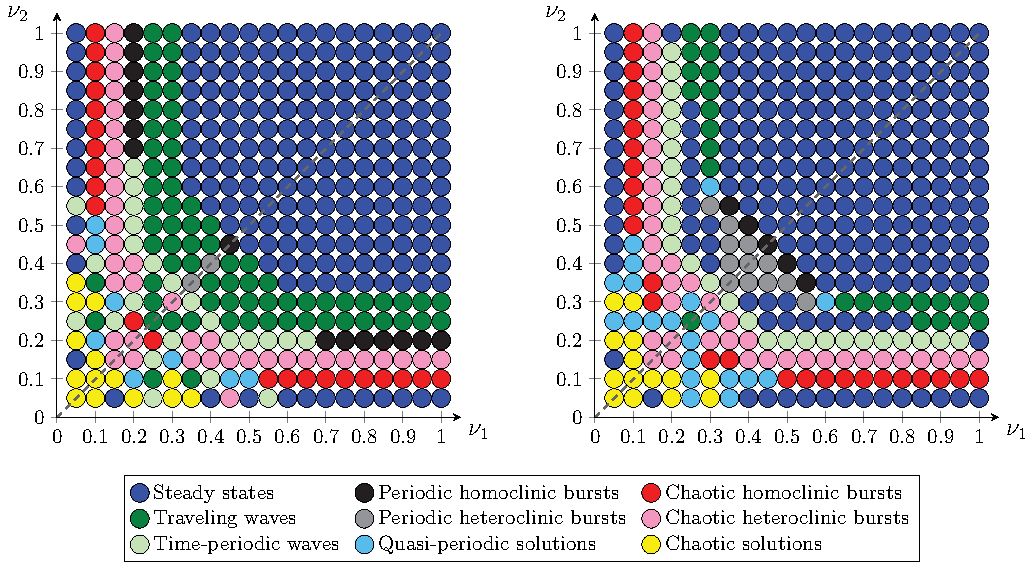
\includegraphics[width=\textwidth]{images/nu1-nu2.pdf}
  \caption{Classification of the different types of solutions for all the values of $\nu_1$ and $\nu_2$ in the interval $[0,1]$ with a discretization of $0.05$. The figure on the left is obtained with the initial condition $u_0(x,y) = \sin(x) + \sin(y) + \sin(x+y)$, and it is taken from \cite{Kalogirou2015}. The figure on the right is obtained with the initial condition \cref{eq:initial_condition}.}
  \label{fig:classification_nu1_nu2}
\end{figure}
First we note that both plots are symmetric with respect to the line $\nu_1=\nu_2$ due to the comment that we have done in \cref{sec:intro}. We can observe some similarities in the right part of the plots and also in the bottom left corner which correspond to small values of $\nu_1$ and $\nu_2$.

As many of the bifurcations may appear at slightly different values of $\nu_1$ and $\nu_2$, many of them are hidden by the big discretization that we have used. For example, we can see that in the left diagram, there is a line of black dots when $\nu_2=0.2$ and $0.7\leq \nu_1 \leq 1$ that we do not observe on the right diagram. Because of this, we have performed a more detailed study of the behaviour of the equation in the case $\nu:=\nu_1=\nu_2$ with a discretization of $0.01$. The results are shown in \cref{fig:classification_nu}.

\begin{figure}[ht]
  \centering
  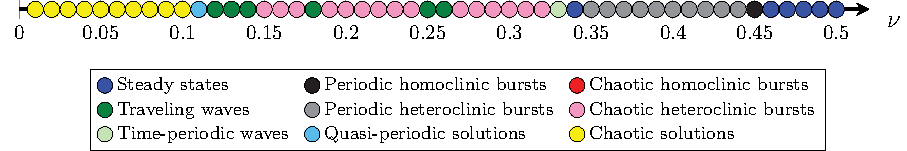
\includegraphics[width=\textwidth]{images/nu1=nu2.pdf}
  \caption{Classification of the different types of solutions for all the values of $\nu$ in the interval $[0,1]$ with a discretization of $0.01$.}
  \label{fig:classification_nu}
\end{figure}
Recall that we have omitted the range $\nu\in(0.5,1]$ because of the monotonous stationary state behaviour of the equation.

In the following sections we will delve into the properties of some solutions shown in those diagrams.
\subsection{Travelling waves}\label{sec:travelling_waves}
We start studying the travelling waves. Observing the right diagram in \cref{fig:classification_nu1_nu2}, we can see that there is an apparently continuous set of solutions around $\nu_2=0.3$ and $0.65\leq \nu_1\leq 1$ containing travelling waves. In the \cref{tab:travelling_waves} we represent the periods of the travelling waves in this interval of $\nu_1$ for fixed $\nu_2=0.3$. Note that the period is inversely proportional to the speed of the wave. Thus, the shorter the period, the faster the travelling wave propagates.

\begin{table}[ht]
  \centering
  \begin{tabular}{|c||cccccccc|}
    \hline
    $\nu_1$ & 0.65   & 0.7    & 0.75   & 0.8    & 0.85   & 0.9    & 0.95   & 1      \\ \hline
    Period  & 39.673 & 42.725 & 45.777 & 48.830 & 51.882 & 54.934 & 57.986 & 61.037 \\
    \hline
  \end{tabular}
  \caption{Periods of the travelling waves for fixed $\nu_2=0.3$ and different values of $\nu_1$.}
  \label{tab:travelling_waves}
\end{table}
What the reader may observe a decrease on the period as $\nu_1$ decreases. In the \cref{fig:sections_tw} we show three equally spaced sections of the travelling wave corresponding to $\nu_1=0.85$ and $\nu_2=0.3$.

\begin{figure}[ht]
  \centering
  \begin{subfigure}[b]{0.32\textwidth}
    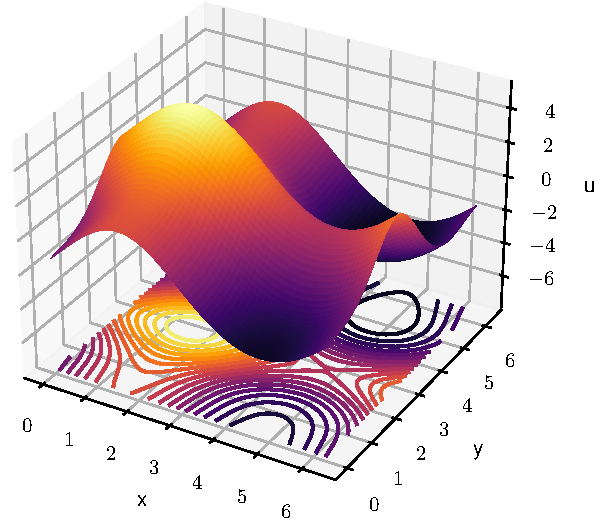
\includegraphics[width=\textwidth]{images/slice_nu1_0.85_nu2_0.3_time_900.0.pdf}
    \caption{$t=900$}
  \end{subfigure}\hfill
  \begin{subfigure}[b]{0.32\textwidth}
    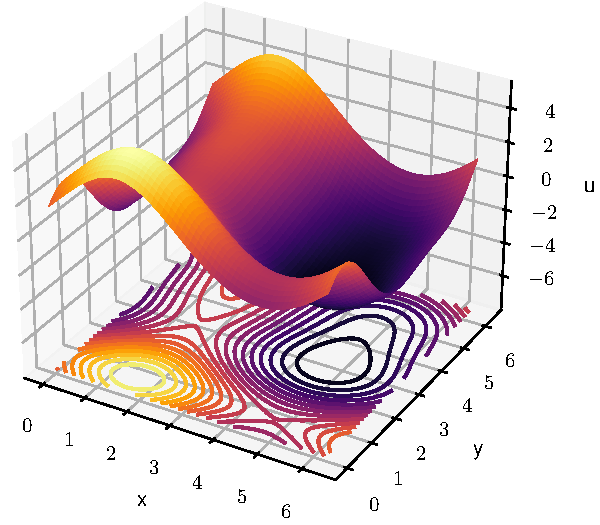
\includegraphics[width=\textwidth]{images/slice_nu1_0.85_nu2_0.3_time_917.294.pdf}
    \caption{$t=917.294$}
  \end{subfigure}\hfill
  \begin{subfigure}[b]{0.32\textwidth}
    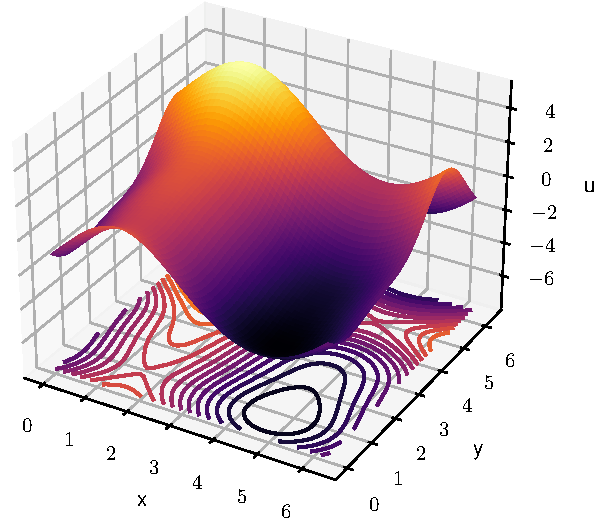
\includegraphics[width=\textwidth]{images/slice_nu1_0.85_nu2_0.3_time_934.588.pdf}
    \caption{$t=934.588$}
  \end{subfigure}
  \caption{Sections of the travelling wave with $\nu_1=0.85$ and $\nu_2=0.3$ at different times.}
  \label{fig:sections_tw}
\end{figure}
The quasi-periodic travelling wave solution that we can observe in \cref{fig:classification_nu1_nu2} is a sign of approaching a bifurcation point between travelling waves and periodic bursts, and maybe other types of solutions. We do not have an analytical proof of this, but only numerical experiments. In \cref{fig:qp_tw} we show the evolution of a particular particle situated at $(\pi,\pi)$ for $\nu_1=0.65$ and $\nu_2=0.3$.

\begin{figure}[ht]
  \centering
  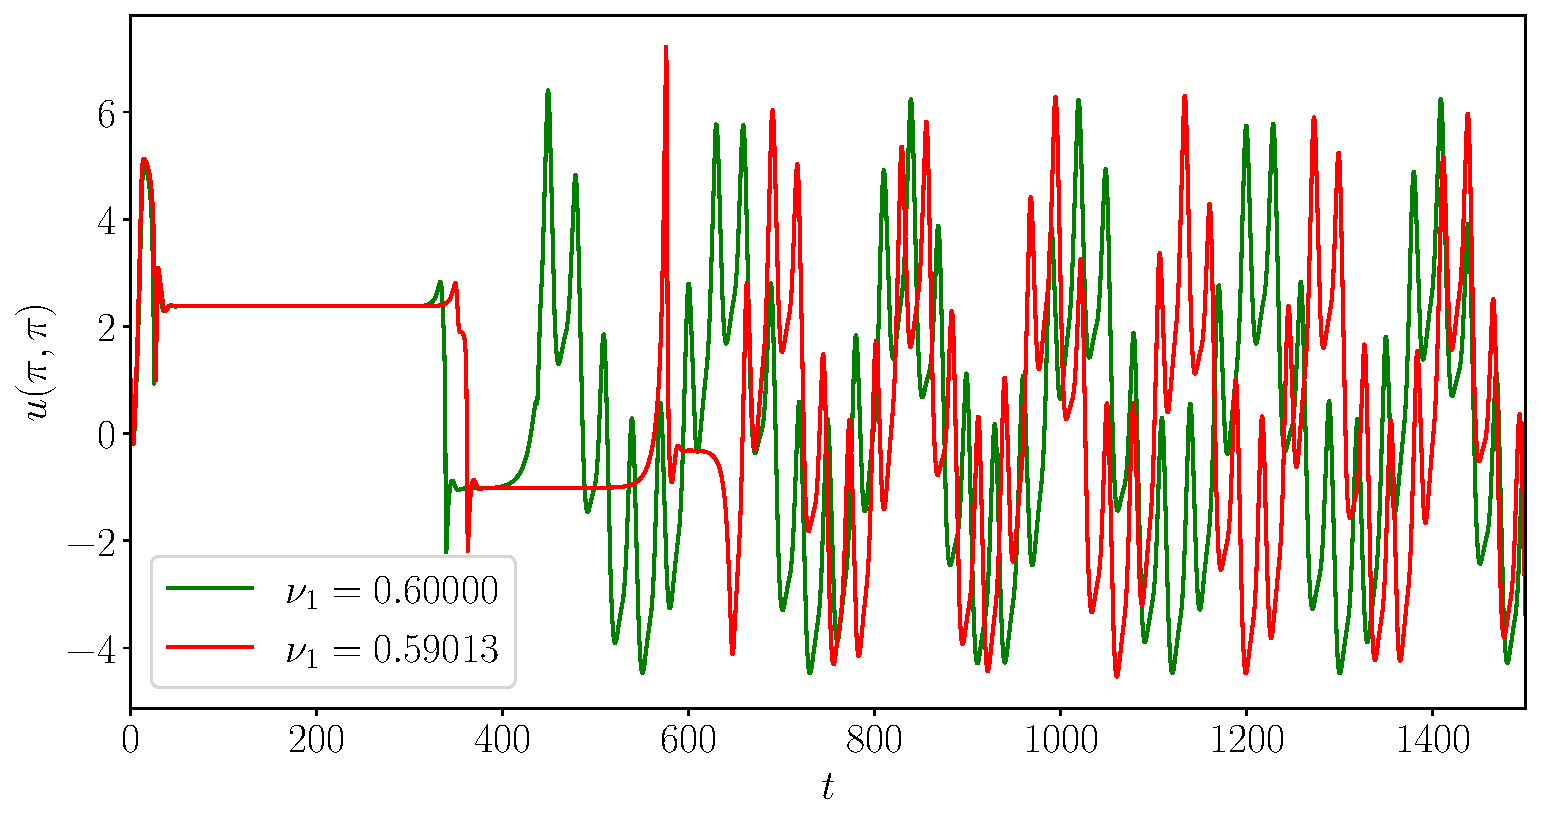
\includegraphics[width=0.7\textwidth]{images/qp_tw.pdf}
  \caption{Evolution of $u(\pi,\pi)$ as a function of time for $\nu_1=0.65$ and $\nu_2=0.3$.}
  \label{fig:qp_tw}
\end{figure}
We let the reader extract their own conclusions when comparing this figure with ????????????? (POSAR HETEROCLINIC).
\subsection{Time periodic waves}\label{sec:time_periodic_waves}
We now move on to the time periodic waves. We can do a similar experiment as in \cref{sec:travelling_waves} and reproduce the periods of the time periodic waves for fixed $\nu_2=0.2$ and $0.45\leq \nu_1\leq 0.95$, as shown in \cref{fig:classification_nu1_nu2}. The results are shown in \cref{tab:time_periodic_waves}.

\begin{table}[ht]
  \centering
  \begin{tabular}{|c||ccccccccccc|}
    \hline
    $\nu_1$ & 0.45  & 0.5   & 0.55  & 0.6   & 0.65  & 0.7   & 0.75  & 0.8   & 0.85  & 0.9   & 0.95  \\ \hline
    Period  & 5.364 & 5.081 & 5.134 & 5.328 & 5.588 & 5.889 & 6.221 & 6.580 & 6.967 & 7.379 & 7.789 \\
    \hline
  \end{tabular}
  \caption{Periods of the time periodic waves for fixed $\nu_2=0.2$ and different values of $\nu_1$.}
  \label{tab:time_periodic_waves}
\end{table}
Again, the periods are decreasing as $\nu_1$ decreases except in the last value of $\nu_1=0.45$, where we observe a sudden increase in the period. We may suspect that this reason has to do with the proximity of a bifurcation point between time periodic waves and bursts. As a pure curiosity, we note that these periods are much smaller than the periods of the travelling waves in \cref{tab:travelling_waves}.

We now display some sections of the time periodic wave corresponding to $\nu_1=0.35$ and $\nu_2=0.3$ in \cref{fig:sections_tp}.

\begin{figure}
  \centering
  \begin{subfigure}[ht]{0.32\textwidth}
    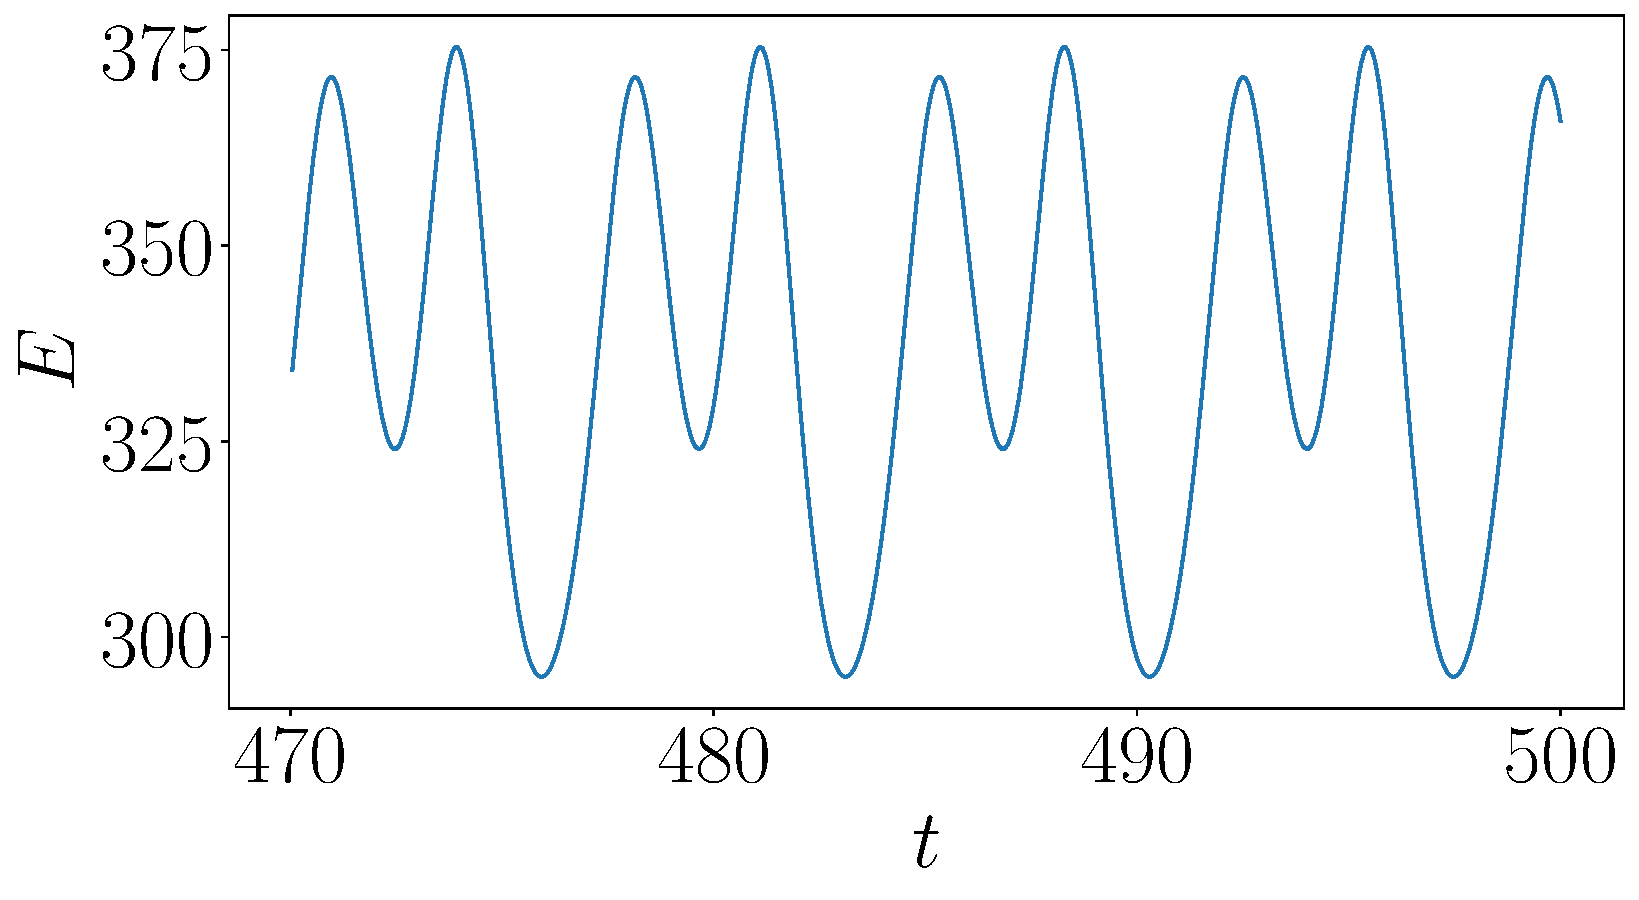
\includegraphics[width=\textwidth]{images/tp_energy.pdf}
    \caption{Energy of the solution as a function of time.}
  \end{subfigure}\hfill
  \begin{subfigure}[ht]{0.32\textwidth}
    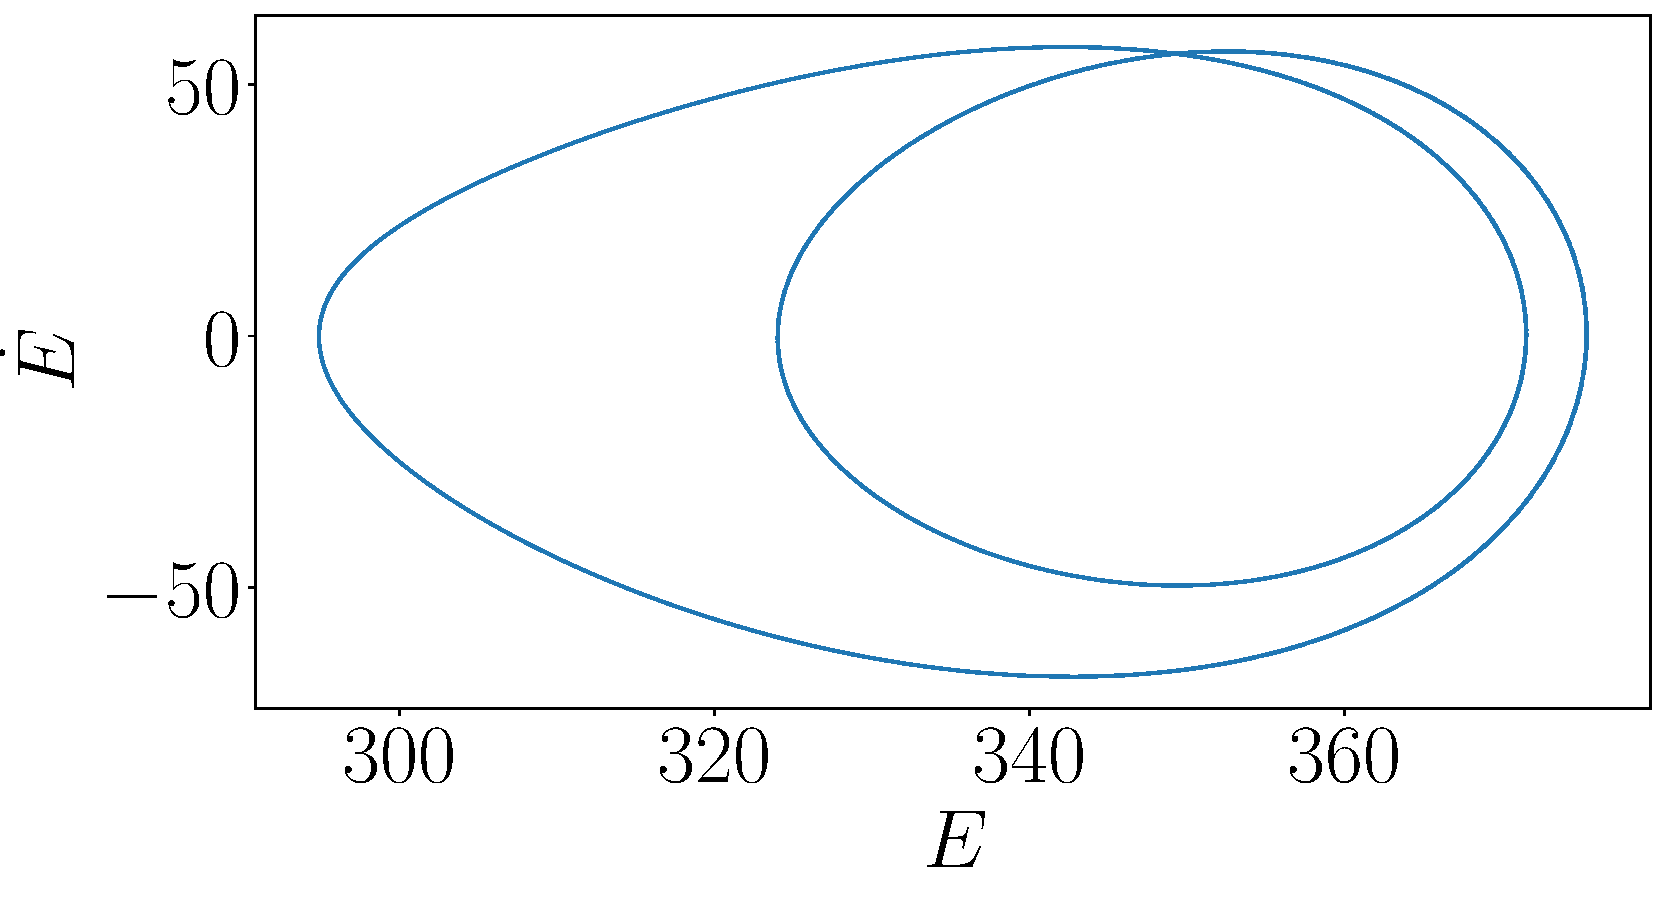
\includegraphics[width=\textwidth]{images/tp_energy_phase.pdf}
    \caption{Phase space $(E(t), \dot{E}(t))$.}
    \label{fig:tp_energy_phase}
  \end{subfigure}\hfill
  \begin{subfigure}[ht]{0.32\textwidth}
    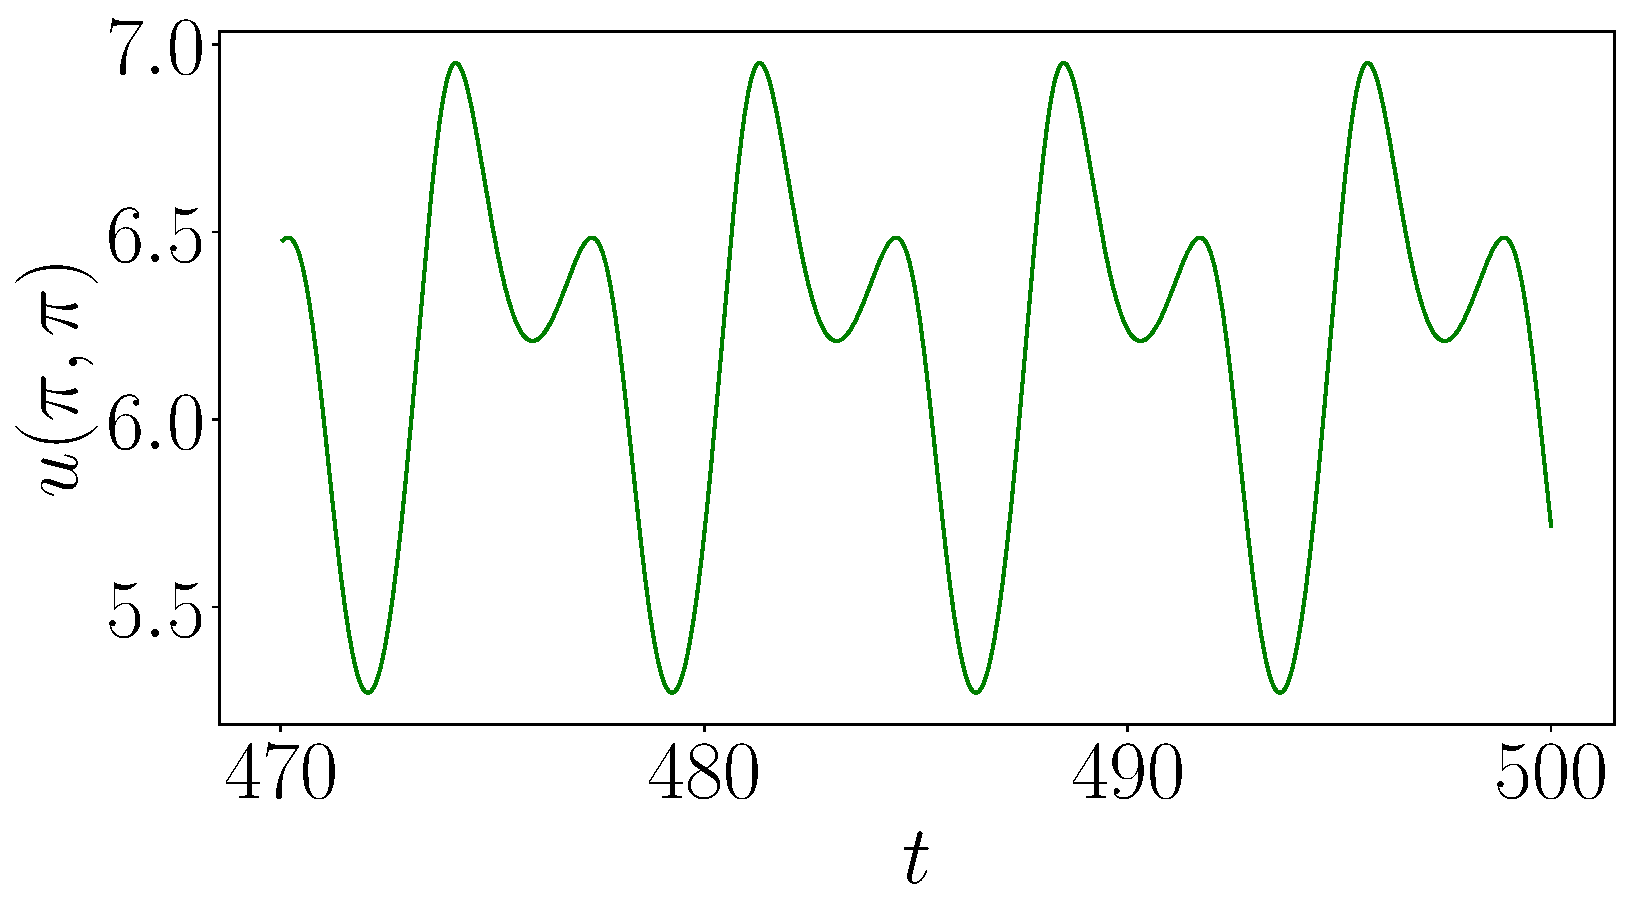
\includegraphics[width=\textwidth]{images/tp_u_pi_pi.pdf}
    \caption{Evolution of $u(\pi,\pi)$ as a function of time.}
  \end{subfigure}\\
  \begin{subfigure}[ht]{0.24\textwidth}
    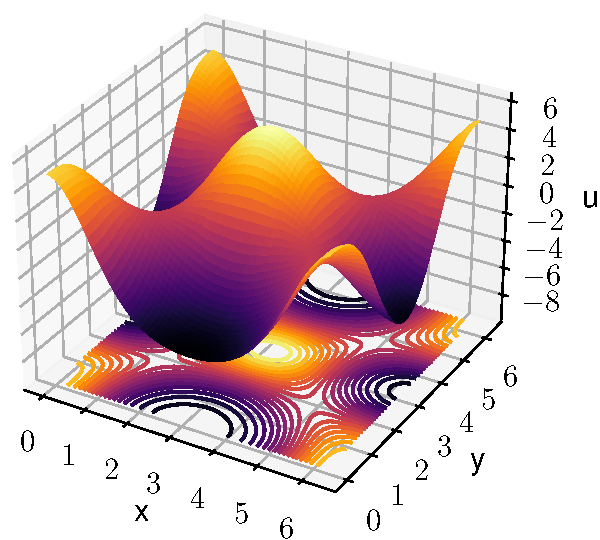
\includegraphics[width=\textwidth]{images/slice_nu1_0.35_nu2_0.3_time_490.24.pdf}
    \caption{$t=490.24$}
  \end{subfigure}\hfill
  \begin{subfigure}[ht]{0.24\textwidth}
    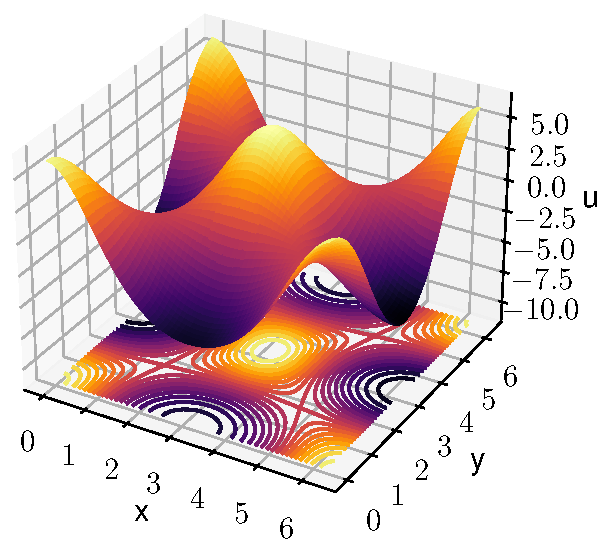
\includegraphics[width=\textwidth]{images/slice_nu1_0.35_nu2_0.3_time_491.7.pdf}
    \caption{$t=491.7$}
  \end{subfigure}\hfill
  \begin{subfigure}[ht]{0.24\textwidth}
    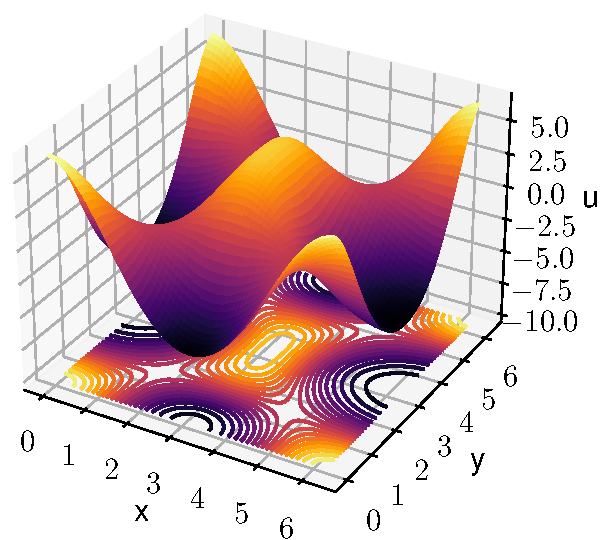
\includegraphics[width=\textwidth]{images/slice_nu1_0.35_nu2_0.3_time_493.61.pdf}
    \caption{$t=493.61$}
  \end{subfigure}\hfill
  \begin{subfigure}[ht]{0.24\textwidth}
    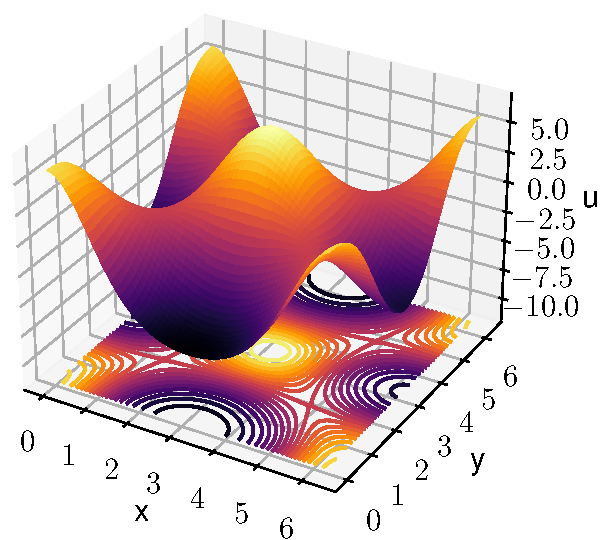
\includegraphics[width=\textwidth]{images/slice_nu1_0.35_nu2_0.3_time_495.62.pdf}
    \caption{$t=495.62$}
  \end{subfigure}
  \caption{Time periodic wave with $\nu_1=0.35$ and $\nu_2=0.3$. On the top we show the energy of the solution as a function of time, its phase space $(E(t), \dot{E}(t))$ and the evolution of $u(\pi,\pi)$ as a function of time. On the bottom we display the solution at each of the four different extrema points of the energy in one period.}
\end{figure}
We should make a point in the phase space $(E(t), \dot{E}(t))$ of \cref{fig:tp_energy_phase}. We can observe that the orbit autointersects itself, which may seem to be a contradiction with the unicity of solution. However, we note that the differential system is not autonomous, and so autointersections are allowed.
\subsection{Periodic bursts}\label{sec:periodic_bursts}
The last type of periodic solutions that remains to be studied are the periodic bursts. In \cref{fig:burst} we show the two different kind of burst that we may encounter in the 2D-KS equation: homoclinic bursts and heteroclinic bursts.

\begin{figure}[ht]
  \centering
  \begin{subfigure}[ht]{0.45\textwidth}
    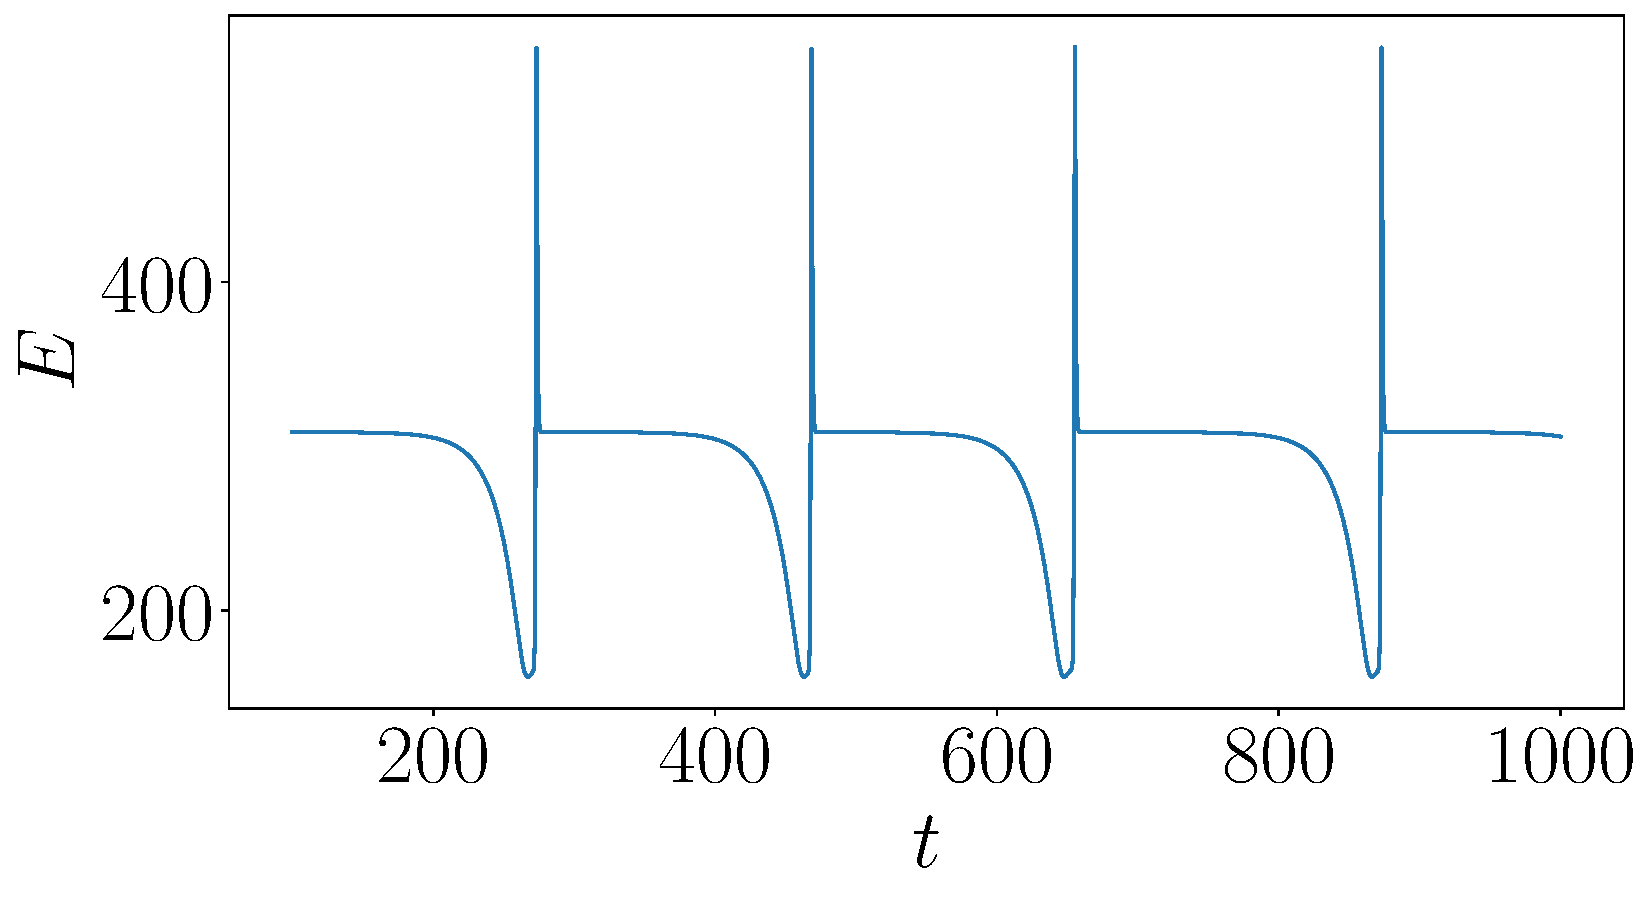
\includegraphics[width=\textwidth]{images/homo_burst.pdf}
    \caption{Evolution of the energy of the homoclinic bursts corresponding to parameters $\nu_1=\nu_2=0.45$.}
  \end{subfigure}\hfill
  \begin{subfigure}[ht]{0.45\textwidth}
    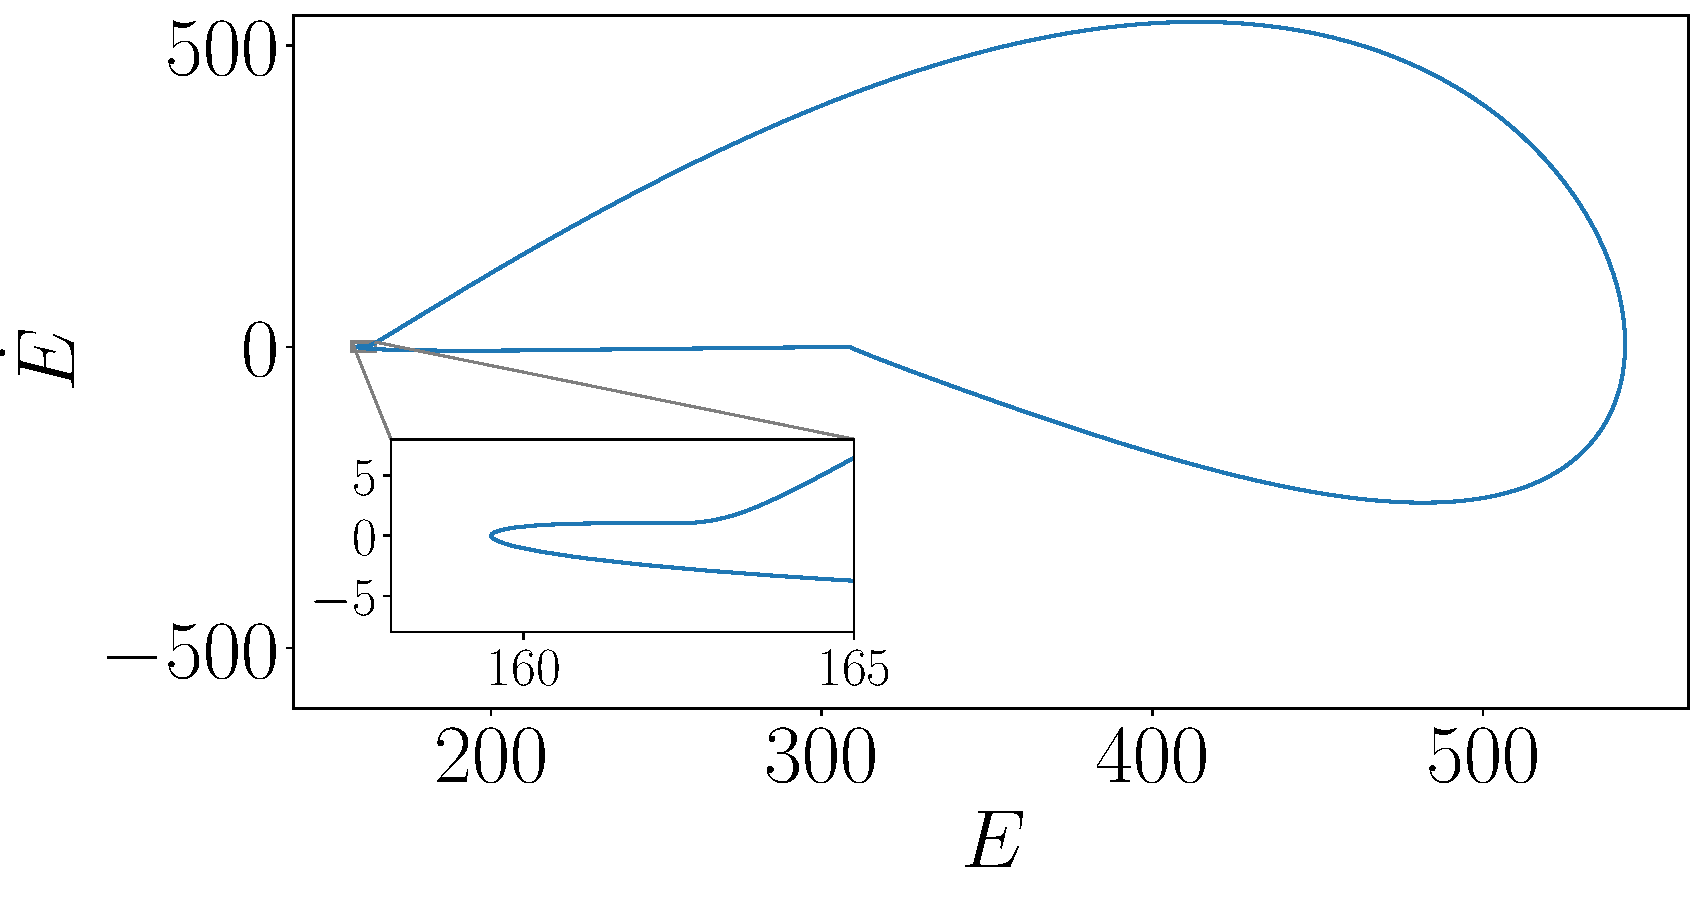
\includegraphics[width=\textwidth]{images/homo_burst_phase.pdf}
    \caption{Phase space $(E(t), \dot{E}(t))$ of the homoclinic bursts corresponding to parameters $\nu_1=\nu_2=0.45$.}
  \end{subfigure}\\
  \begin{subfigure}[ht]{0.45\textwidth}
    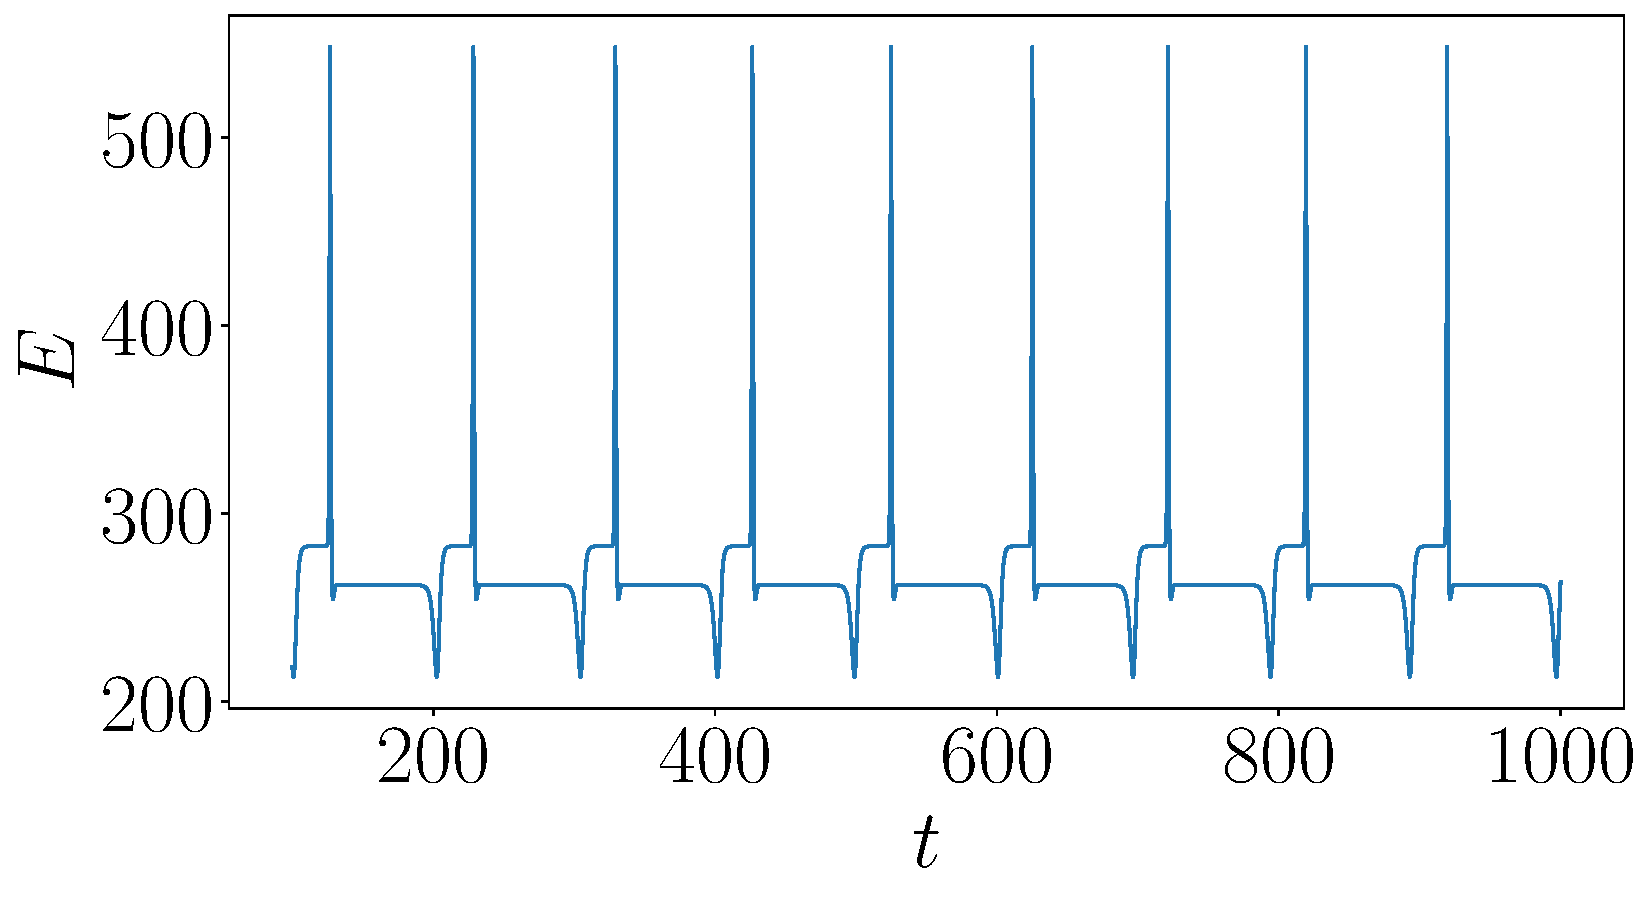
\includegraphics[width=\textwidth]{images/hetero_burst.pdf}
    \caption{Evolution of the energy of the heteroclinic bursts corresponding to parameters $\nu_1=\nu_2=0.4$.}
  \end{subfigure}\hfill
  \begin{subfigure}[ht]{0.45\textwidth}
    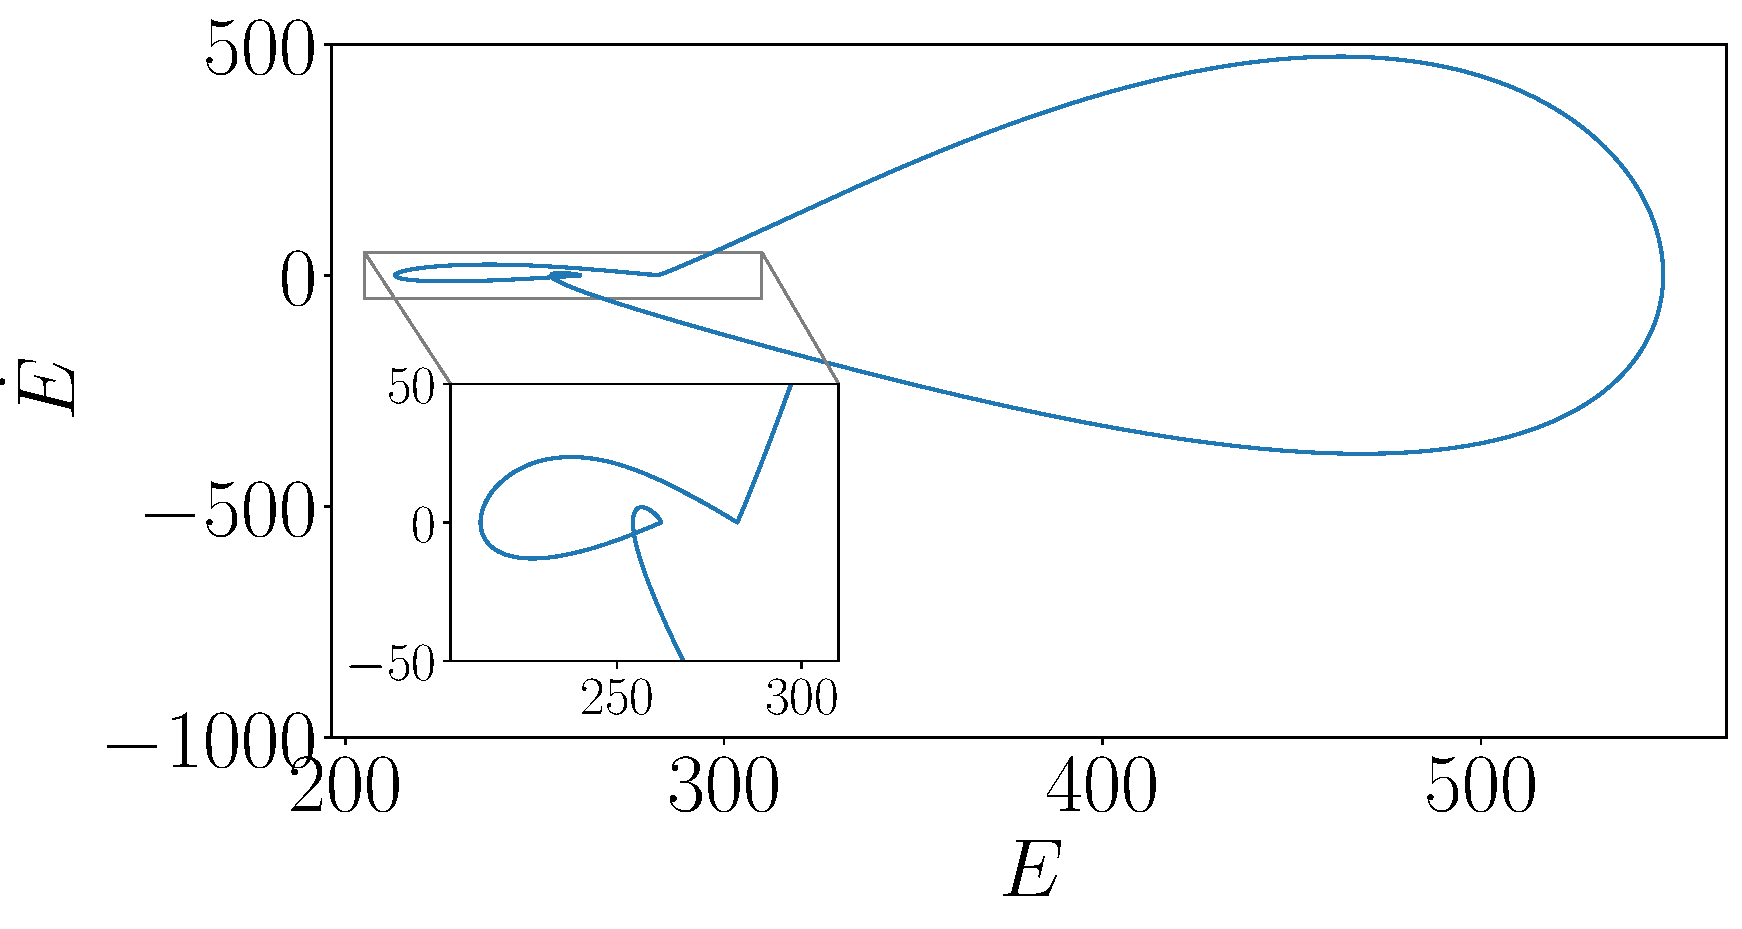
\includegraphics[width=\textwidth]{images/hetero_burst_phase.pdf}
    \caption{Phase space $(E(t), \dot{E}(t))$ of the heteroclinic bursts corresponding to parameters $\nu_1=\nu_2=0.4$.}
  \end{subfigure}
  \caption{Types of bursts.}
  \label{fig:burst}
\end{figure}

\subsection{Quasi-periodicity and chaotic behaviour}\label{sec:chaotic}
Last but not least, we will now expose some of the chaotic behaviours that we have found. It is worth noting that in order to compute with the same accuracy as before the chaotic solutions that appear for small $\nu_1$ and $\nu_2$, we had to decrease the time step to $h=0.001$ and increase the spatial resolution to $N_x=N_y=128$.

We start with the quasi-periodic solutions. In \cref{fig:qp} we show the phase space $(E(t), \dot{E}(t))$ and the return map $(E_n,E_{n+1})$ for $\nu_1=0.25$ and $\nu_2=0.2$.

\begin{figure}[ht]
  \centering
  \begin{subfigure}[ht]{0.45\textwidth}
    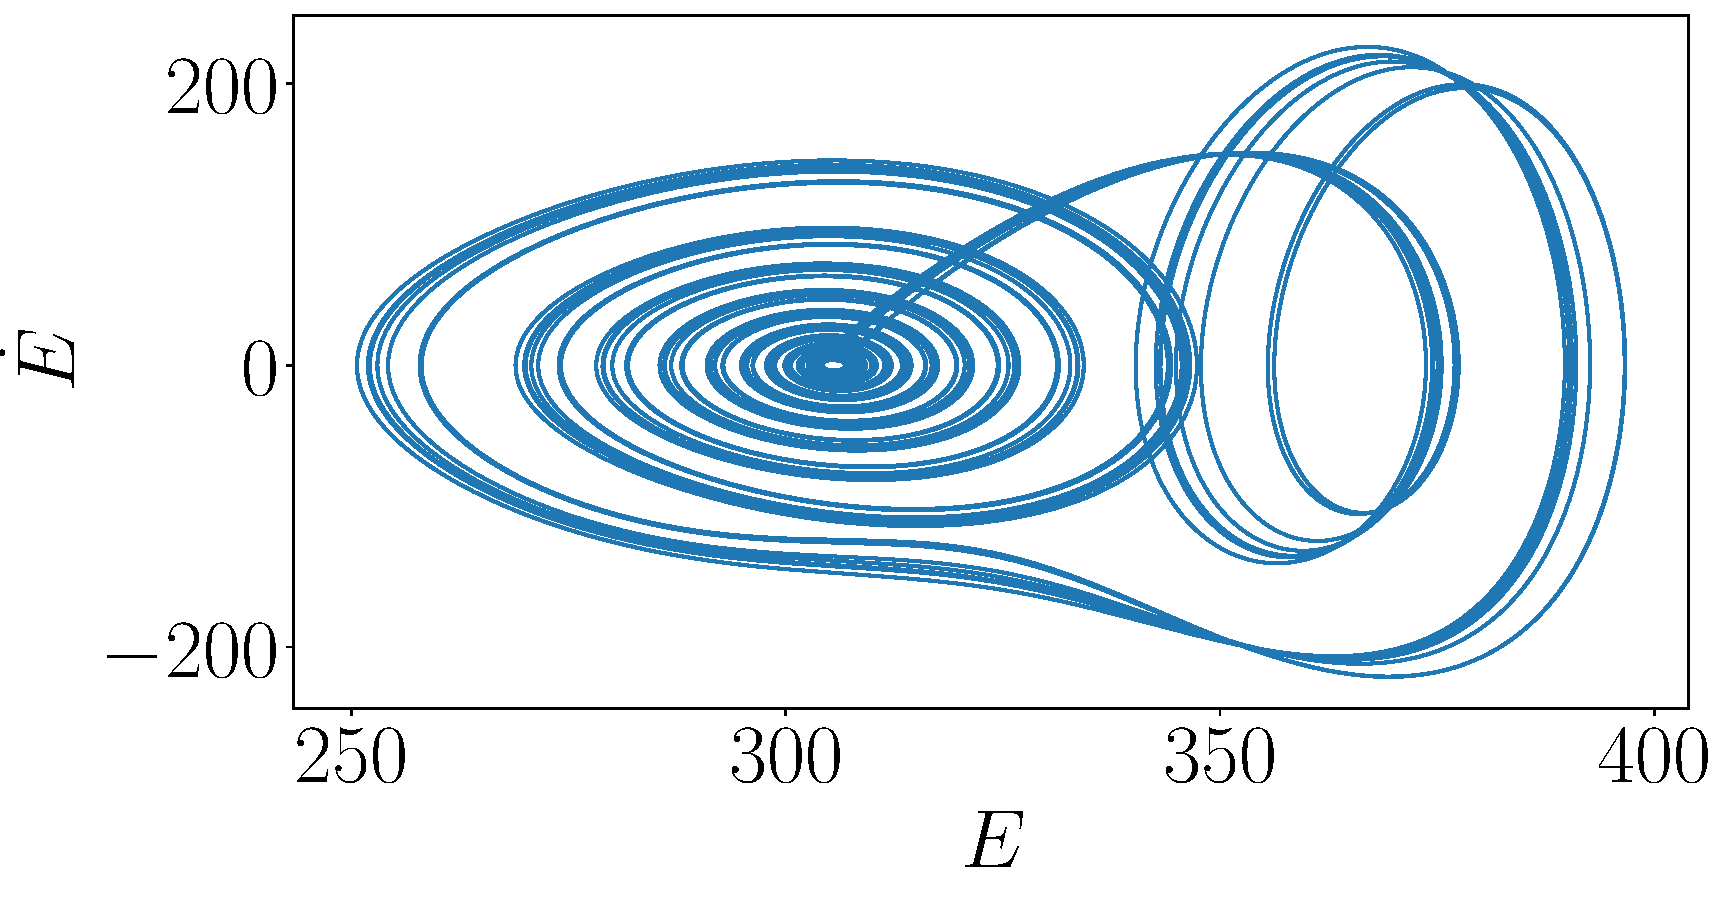
\includegraphics[width=\textwidth]{images/qp_phase.pdf}
    \caption{Phase space $(E(t), \dot{E}(t))$}
  \end{subfigure}\hfill
  \begin{subfigure}[ht]{0.45\textwidth}
    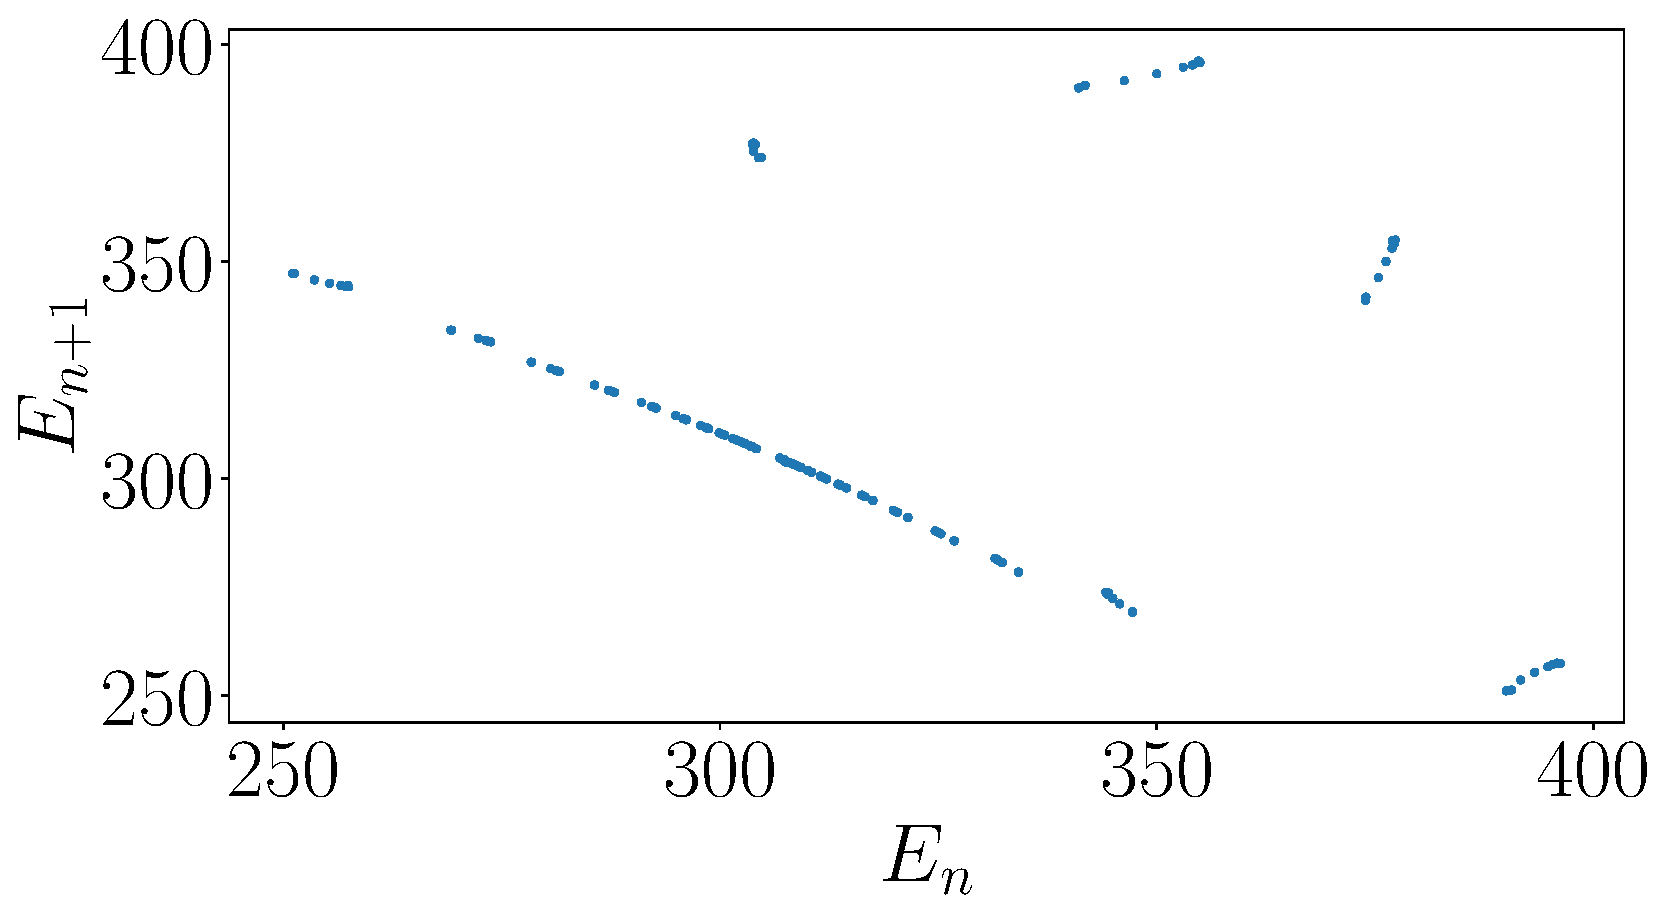
\includegraphics[width=\textwidth]{images/qp_return.pdf}
    \caption{Return map $(E_n,E_{n+1})$}
  \end{subfigure}
  \caption{Quasi-periodic solution corresponding to parameters $\nu_1=0.25$ and $\nu_2=0.2$.}
  \label{fig:qp}
\end{figure}
From the images we can clearly observe the \emph{quasi} periodicity of the solution as the orbit in the phase space $(E(t), \dot{E}(t))$ does not exactly close into itself once it has completed a \emph{period}. From the experiments we can also conclude that quasi-periodic solutions come, among other cases, before bursts and after travelling waves. Thus, some of them still exhibit the property of having constant or almost constant energy.

The following images show chaotic burst. We will not dive into the details of properties of these solutions, as they are relatively similar to the ones studied in \cref{sec:periodic_bursts}, but with more complex behaviour at the beginning of each burst whose accuracy is numerically difficult to control.

\begin{figure}[ht]
  \centering
  \begin{subfigure}[ht]{0.45\textwidth}
    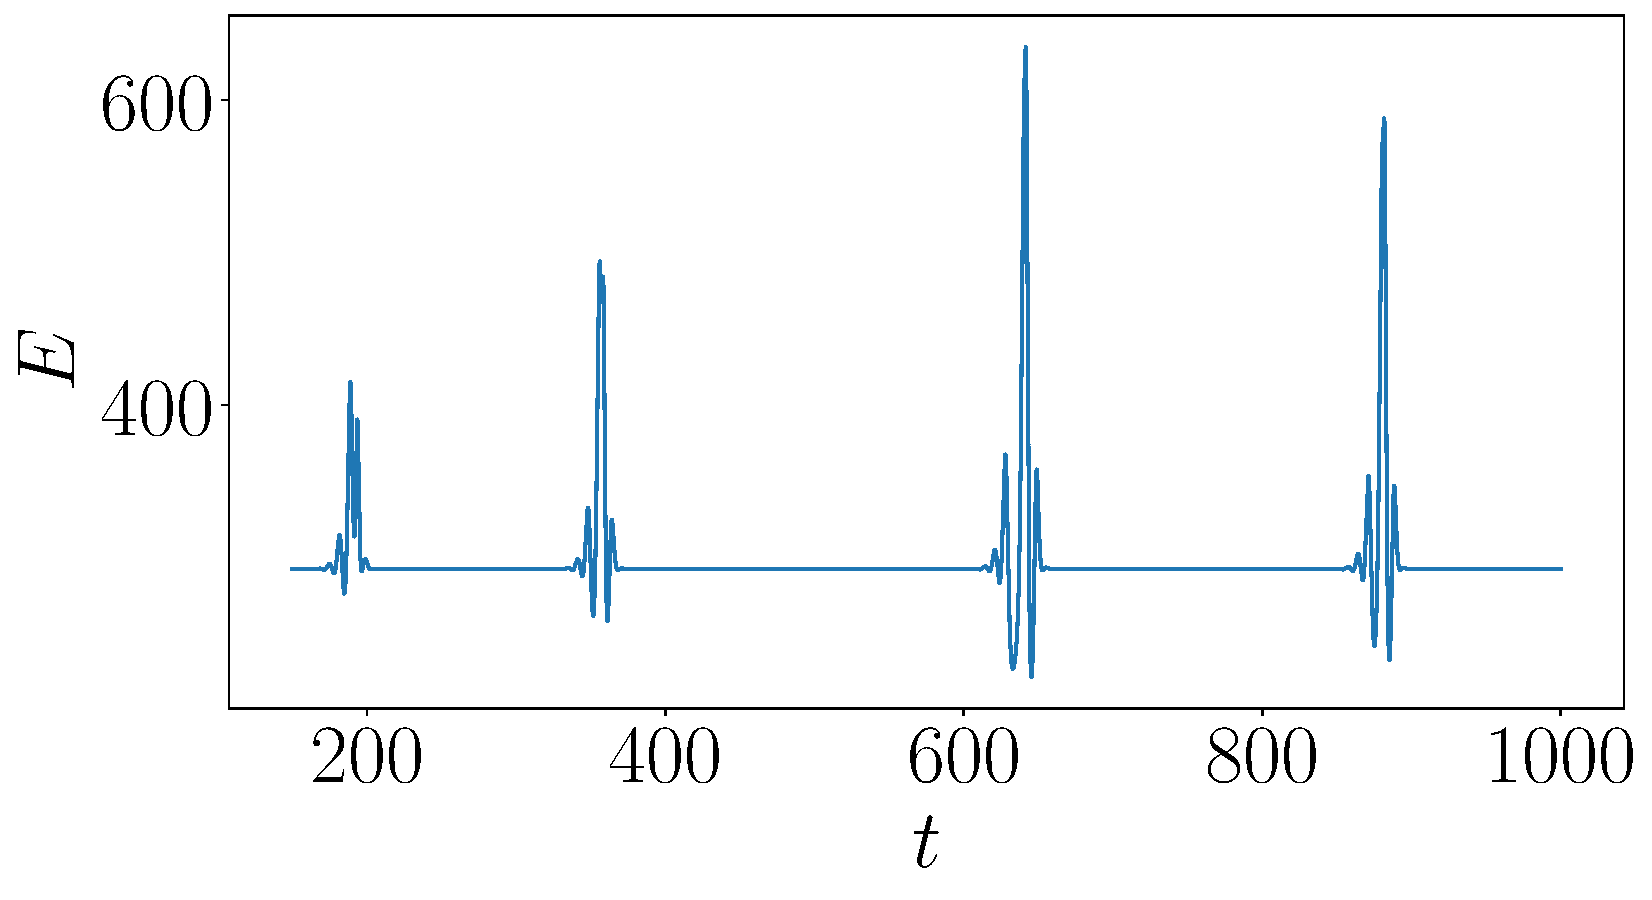
\includegraphics[width=\textwidth]{images/homo_chaotic.pdf}
    \caption{Energy evolution of the chaotic homoclinic bursts corresponding to the solution with parameters $\nu_1=0.75$ and $\nu_2=0.1$.}
  \end{subfigure}\hfill
  \begin{subfigure}[ht]{0.45\textwidth}
    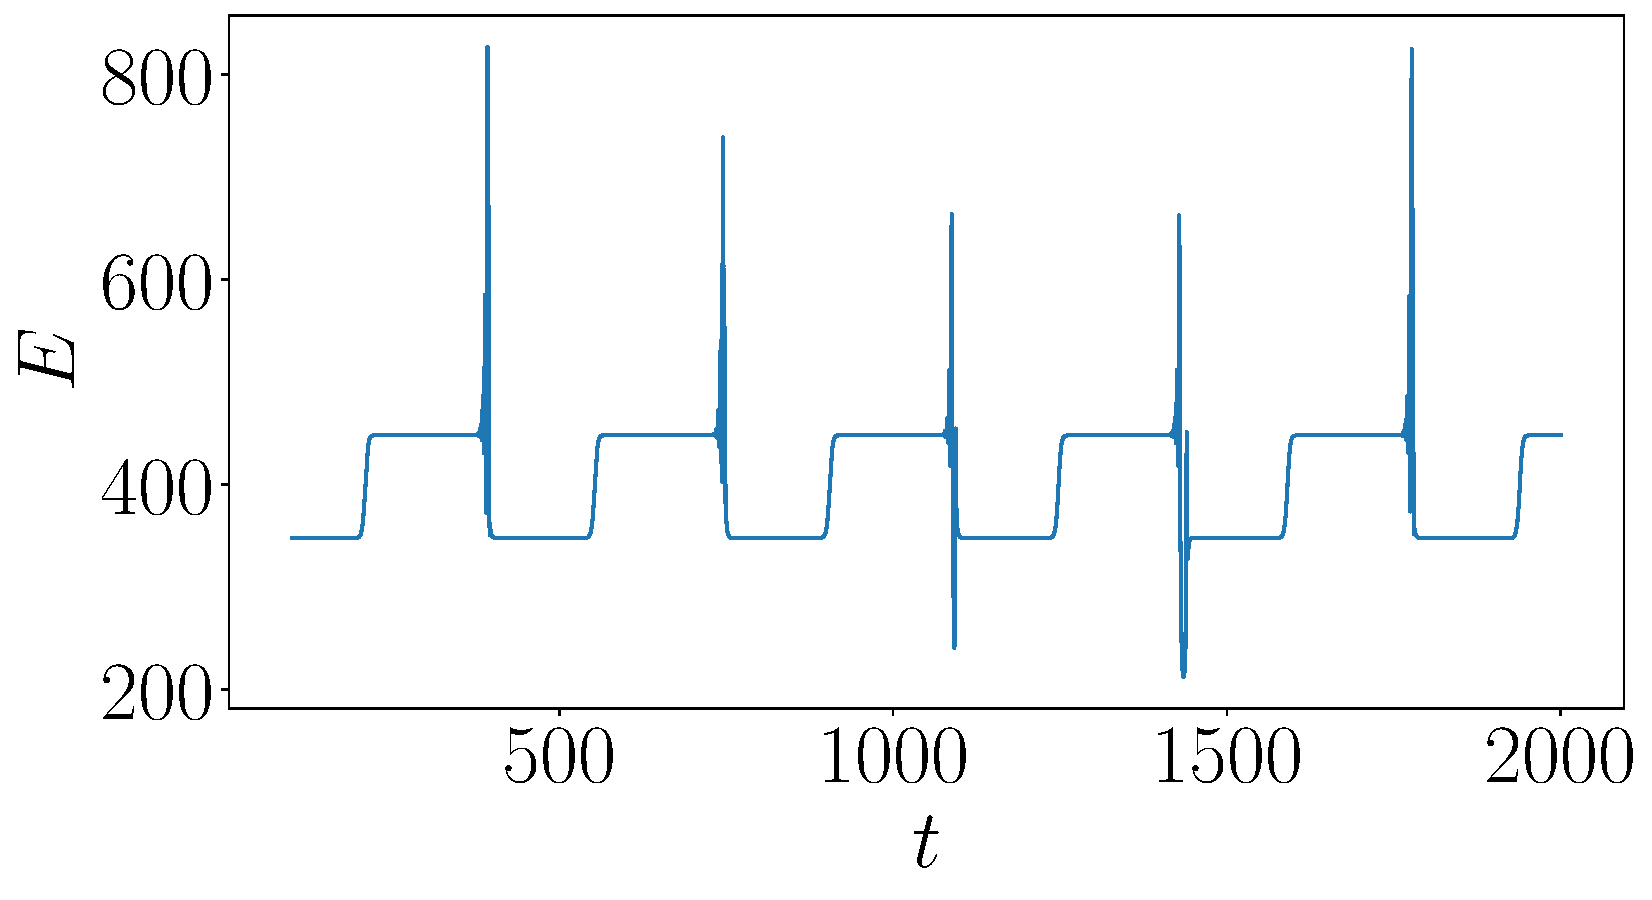
\includegraphics[width=\textwidth]{images/hetero_chaotic.pdf}
    \caption{Energy evolution of the chaotic heteroclinic bursts corresponding to the solution with parameters $\nu_1=0.75$ and $\nu_2=0.15$.}
  \end{subfigure}
  \caption{Chaotic bursts}
  \label{fig:chaotic_burst}
\end{figure}
We can easily observe the roughness of the peaks of the burst in \cref{fig:sec:chaotic_burst}.

We finish this section and this report with displaying some completely chaotic solutions.
\begin{figure}[ht]
  \centering
  \begin{subfigure}[ht]{0.45\textwidth}
    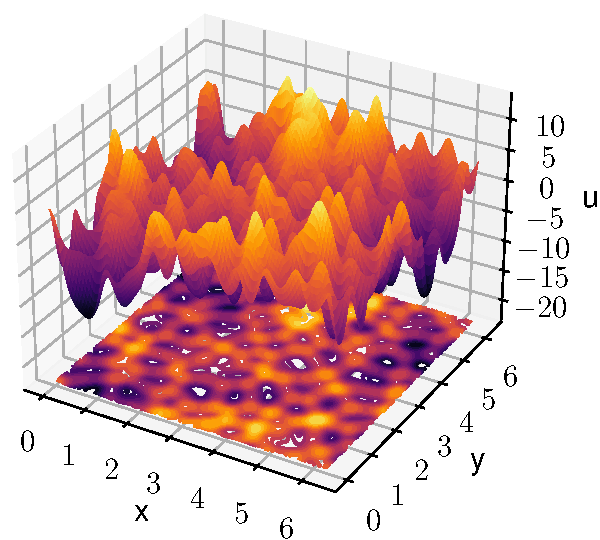
\includegraphics[width=\textwidth]{images/slice_nu1_0.008_nu2_0.008_time_5.0.pdf}
    \caption{Physical solution at $T=5$}
    \label{fig:chaotic_phys}
  \end{subfigure}\hfill
  \begin{subfigure}[ht]{0.45\textwidth}
    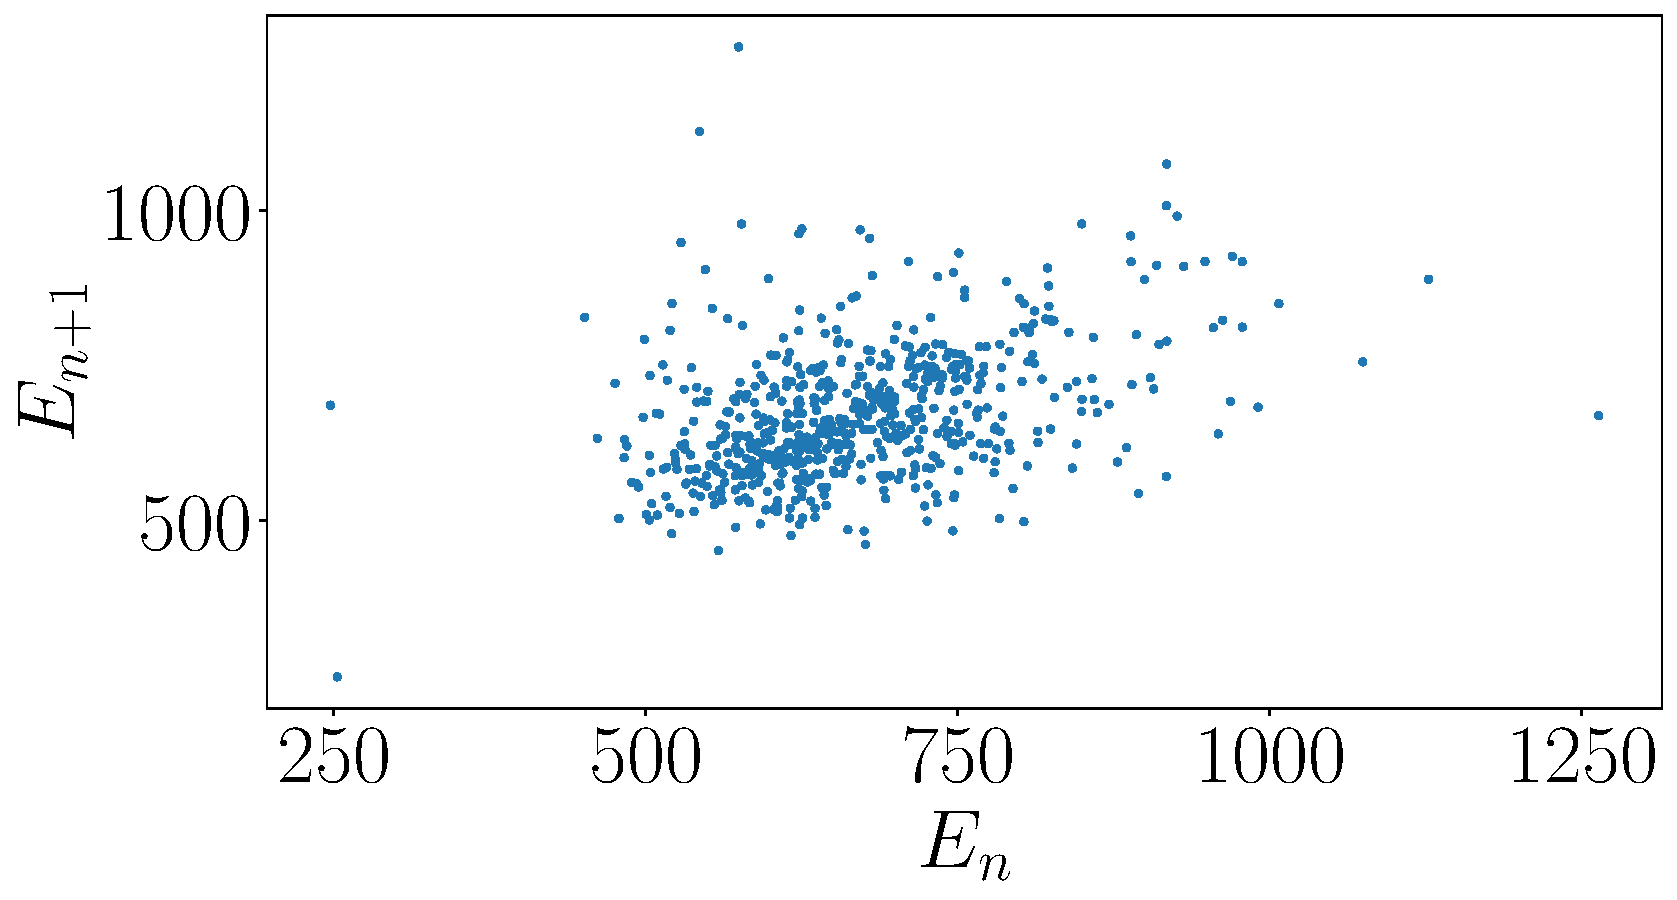
\includegraphics[width=\textwidth]{images/c_return.pdf}
    \caption{Return map $(E_n,E_{n+1})$ of the chaotic solution when intregating the equation in the range $t\in[0,20]$.}
  \end{subfigure}
  \caption{Chaotic solution corresponding to parameters $\nu_1=\nu_2=0.008$}
  \label{fig:chaotic}
\end{figure}
Although from the \cref{fig:chaotic_phys} one may think that there are many large unstable Fourier modes in the solution, the reality is that all the frequencies $(k_x,k_y)$ are less than 12, that is, $k_x,k_y\in\{0,\dots,11\}$. This can be deduced from \cref{eq:linear_stability}, but it only gives the stability in the linear regime. To properly understand the contribution of the different modes, we have computed the amplitude ${k_x}^2+{k_y}^2$ of the Fourier modes and we have represented them in \cref{fig:chaotic_modes}.

\begin{figure}[ht]
  \centering
  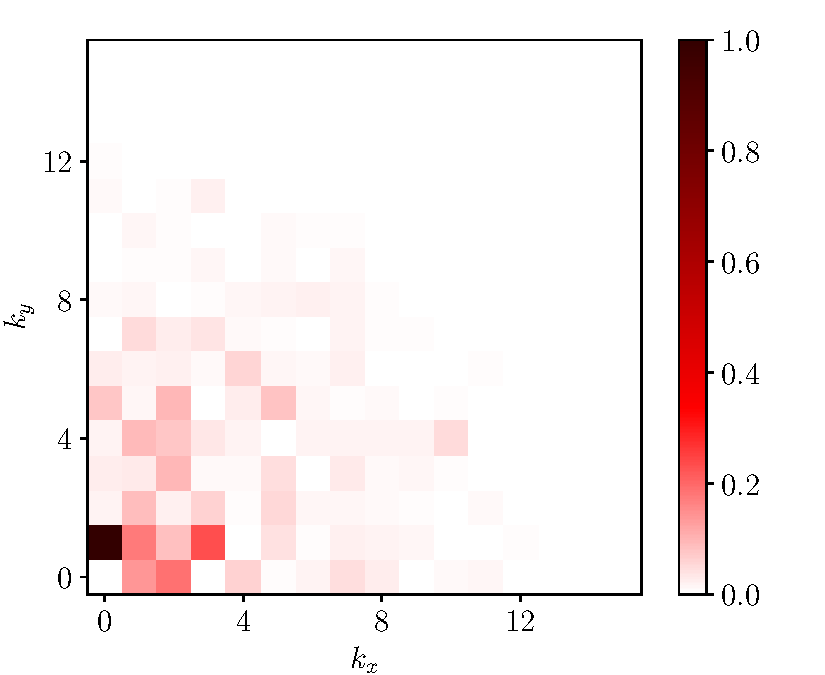
\includegraphics[width=0.5\textwidth]{images/slice_freq_nu1_0.008_nu2_0.008_time_5.0.pdf}
  \caption{Normalized amplitude of the Fourier modes at $T=5$ of the chaotic solution corresponding to parameters $\nu_1=\nu_2=0.008$.}
  \label{fig:chaotic_modes}
\end{figure}
Therefore, we confirm that modes does not go beyond 12 at time $T=5$.
\section{Conclusions}

\phantomsection
\addcontentsline{toc}{section}{References}
\printbibliography
\end{document}













